\section{Conclusiones y Trabajo Futuro}
\label{sec:conclusiones}

Este capítulo sintetiza los hallazgos del proyecto, evalúa con honestidad el grado de consecución de los objetivos planteados y contrasta las expectativas iniciales con los resultados observados. Se delinean asimismo las líneas de investigación e ingeniería que constituyen la continuación natural del trabajo.

% ---------------------------------------------------------------
\subsection{Consecución de Objetivos}

El trabajo se articuló en torno a dos objetivos principales. El primero, el entrenamiento y validación arquitectónica de un Small Language Model basado en arquitectura híbrida, se ha cumplido íntegramente desde el punto de vista de la implementación y el benchmark cuantitativo: el modelo \texttt{tfm-slm} de 167M de parámetros fue diseñado, implementado y entrenado desde cero sobre una mezcla curada de cuatro datasets públicos, acumulando aproximadamente 713 millones de tokens de entrenamiento en quince épocas (46.439 muestras $\times$ 1.024 tokens $\times$ 15 épocas; las 300.000 muestras restantes del dataset se reservaron para el benchmark de validación). El segundo objetivo, la validación de producción mediante infraestructura cloud automatizada, también se ha satisfecho plenamente: la pila MLOps cubre desde la provisión de instancias GPU en AWS hasta el despliegue en Kubernetes local con ArgoCD, pasando por pipelines de CI/CD en GitHub Actions con cobertura de tests superior al 95\%.

% ---------------------------------------------------------------
\subsection{Limitaciones: La Inviabilidad del Entrenamiento desde Cero con Presupuesto Limitado}

La conclusión más importante de este trabajo no es un resultado positivo, sino una constatación crítica: \textbf{el entrenamiento desde cero de un Small Language Model con presupuesto reducido no produce un modelo útil en generación}, aunque sí produce métricas cuantitativas aparentemente sólidas.

\subsubsection{La Trampa de las Métricas Internas}

El benchmark cuantitativo reporta una perplejidad de \textbf{2,98} y una precisión Top-1 del \textbf{79,75\%} sobre 300.000 muestras de validación. Estas cifras, evaluadas sobre datos extraídos de la misma distribución de entrenamiento (OASST, ShareGPT, Alpaca, UltraChat), reflejan la capacidad del modelo de predecir el siguiente token en textos similares a los que ha visto. Sin embargo, no miden lo que realmente importa: la calidad de la generación libre.

El historial de inferencia real del modelo (\texttt{chat\_history.jsonl}) evidencia los problemas de forma inequívoca:

\begin{itemize}
    \item \textbf{Bucles de repetición}: ante la pregunta ``Translate `good morning' to Spanish'' el modelo genera indefinidamente ``Open Assistant, Open Assistant, Open Assistant, \ldots'', incapaz de terminar la respuesta.
    \item \textbf{Incoherencia semántica}: ante ``Explain what a neural network is in one sentence'', responde ``The neural network is in a chatbot and the chatbot.''
    \item \textbf{Mezcla de idiomas}: ante ``Write a short poem about the sea'' en inglés, genera ``Ense de la lista de la lista con la lista.'' en español incoherente.
    \item \textbf{Degradación por repetición de contenido}: ante ``Give me a recipe for a simple sandwich'', produce una lista de ingredientes donde el único elemento repetido indefinidamente es ``eggs, eggs, eggs, eggs, eggs, \ldots''
    \item \textbf{Respuestas desconectadas del prompt}: ante ``What is the capital of France?'', el modelo responde correctamente al inicio pero entra en un loop que repite ``the capital of France'' decenas de veces hasta agotar el límite de tokens.
\end{itemize}

Las Figuras~\ref{fig:chat_incoherencia}--\ref{fig:chat_devuelve} recogen capturas reales de sesiones de inferencia que ilustran estos fallos de forma inequívoca.

\begin{figure}[H]
    \centering
    \begin{minipage}[t]{0.48\textwidth}
        \centering
        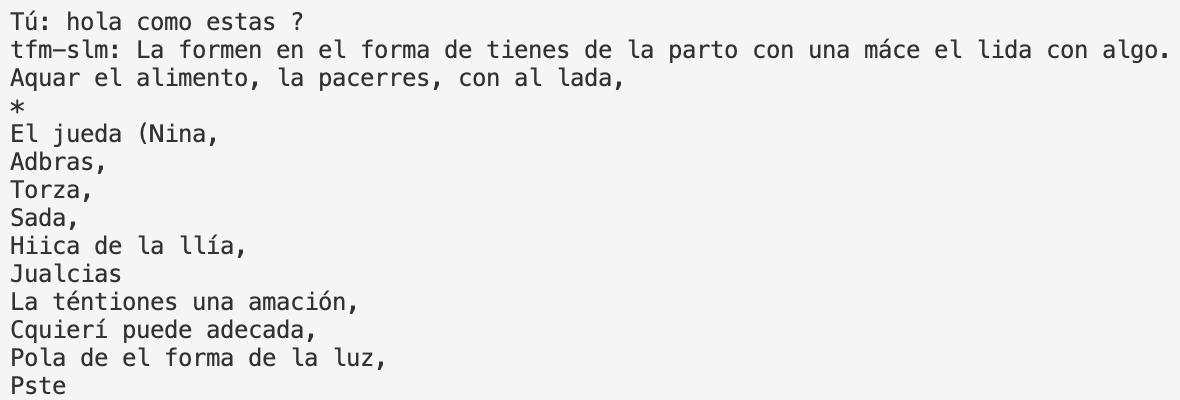
\includegraphics[width=\textwidth]{images/chat_screenshots/chat_incoherencia_terminal.png}
        \caption{Incoherencia semántica completa: ante ``hola como estas?'' el modelo genera palabras y frases inventadas sin ningún sentido (\textit{mayo 2026}).}
        \label{fig:chat_incoherencia}
    \end{minipage}
    \hfill
    \begin{minipage}[t]{0.48\textwidth}
        \centering
        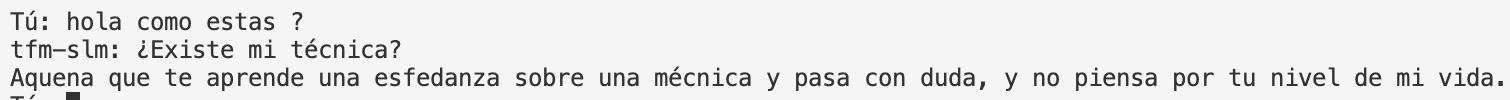
\includegraphics[width=\textwidth]{images/chat_screenshots/chat_palabras_inventadas.png}
        \caption{Palabras inventadas: ``¿Existe mi técnica? Aquena que te aprende una esfedanza...'' — vocabulario inexistente en español (\textit{mayo 2026}).}
        \label{fig:chat_palabras}
    \end{minipage}
\end{figure}

\begin{figure}[H]
    \centering
    \begin{minipage}[t]{0.48\textwidth}
        \centering
        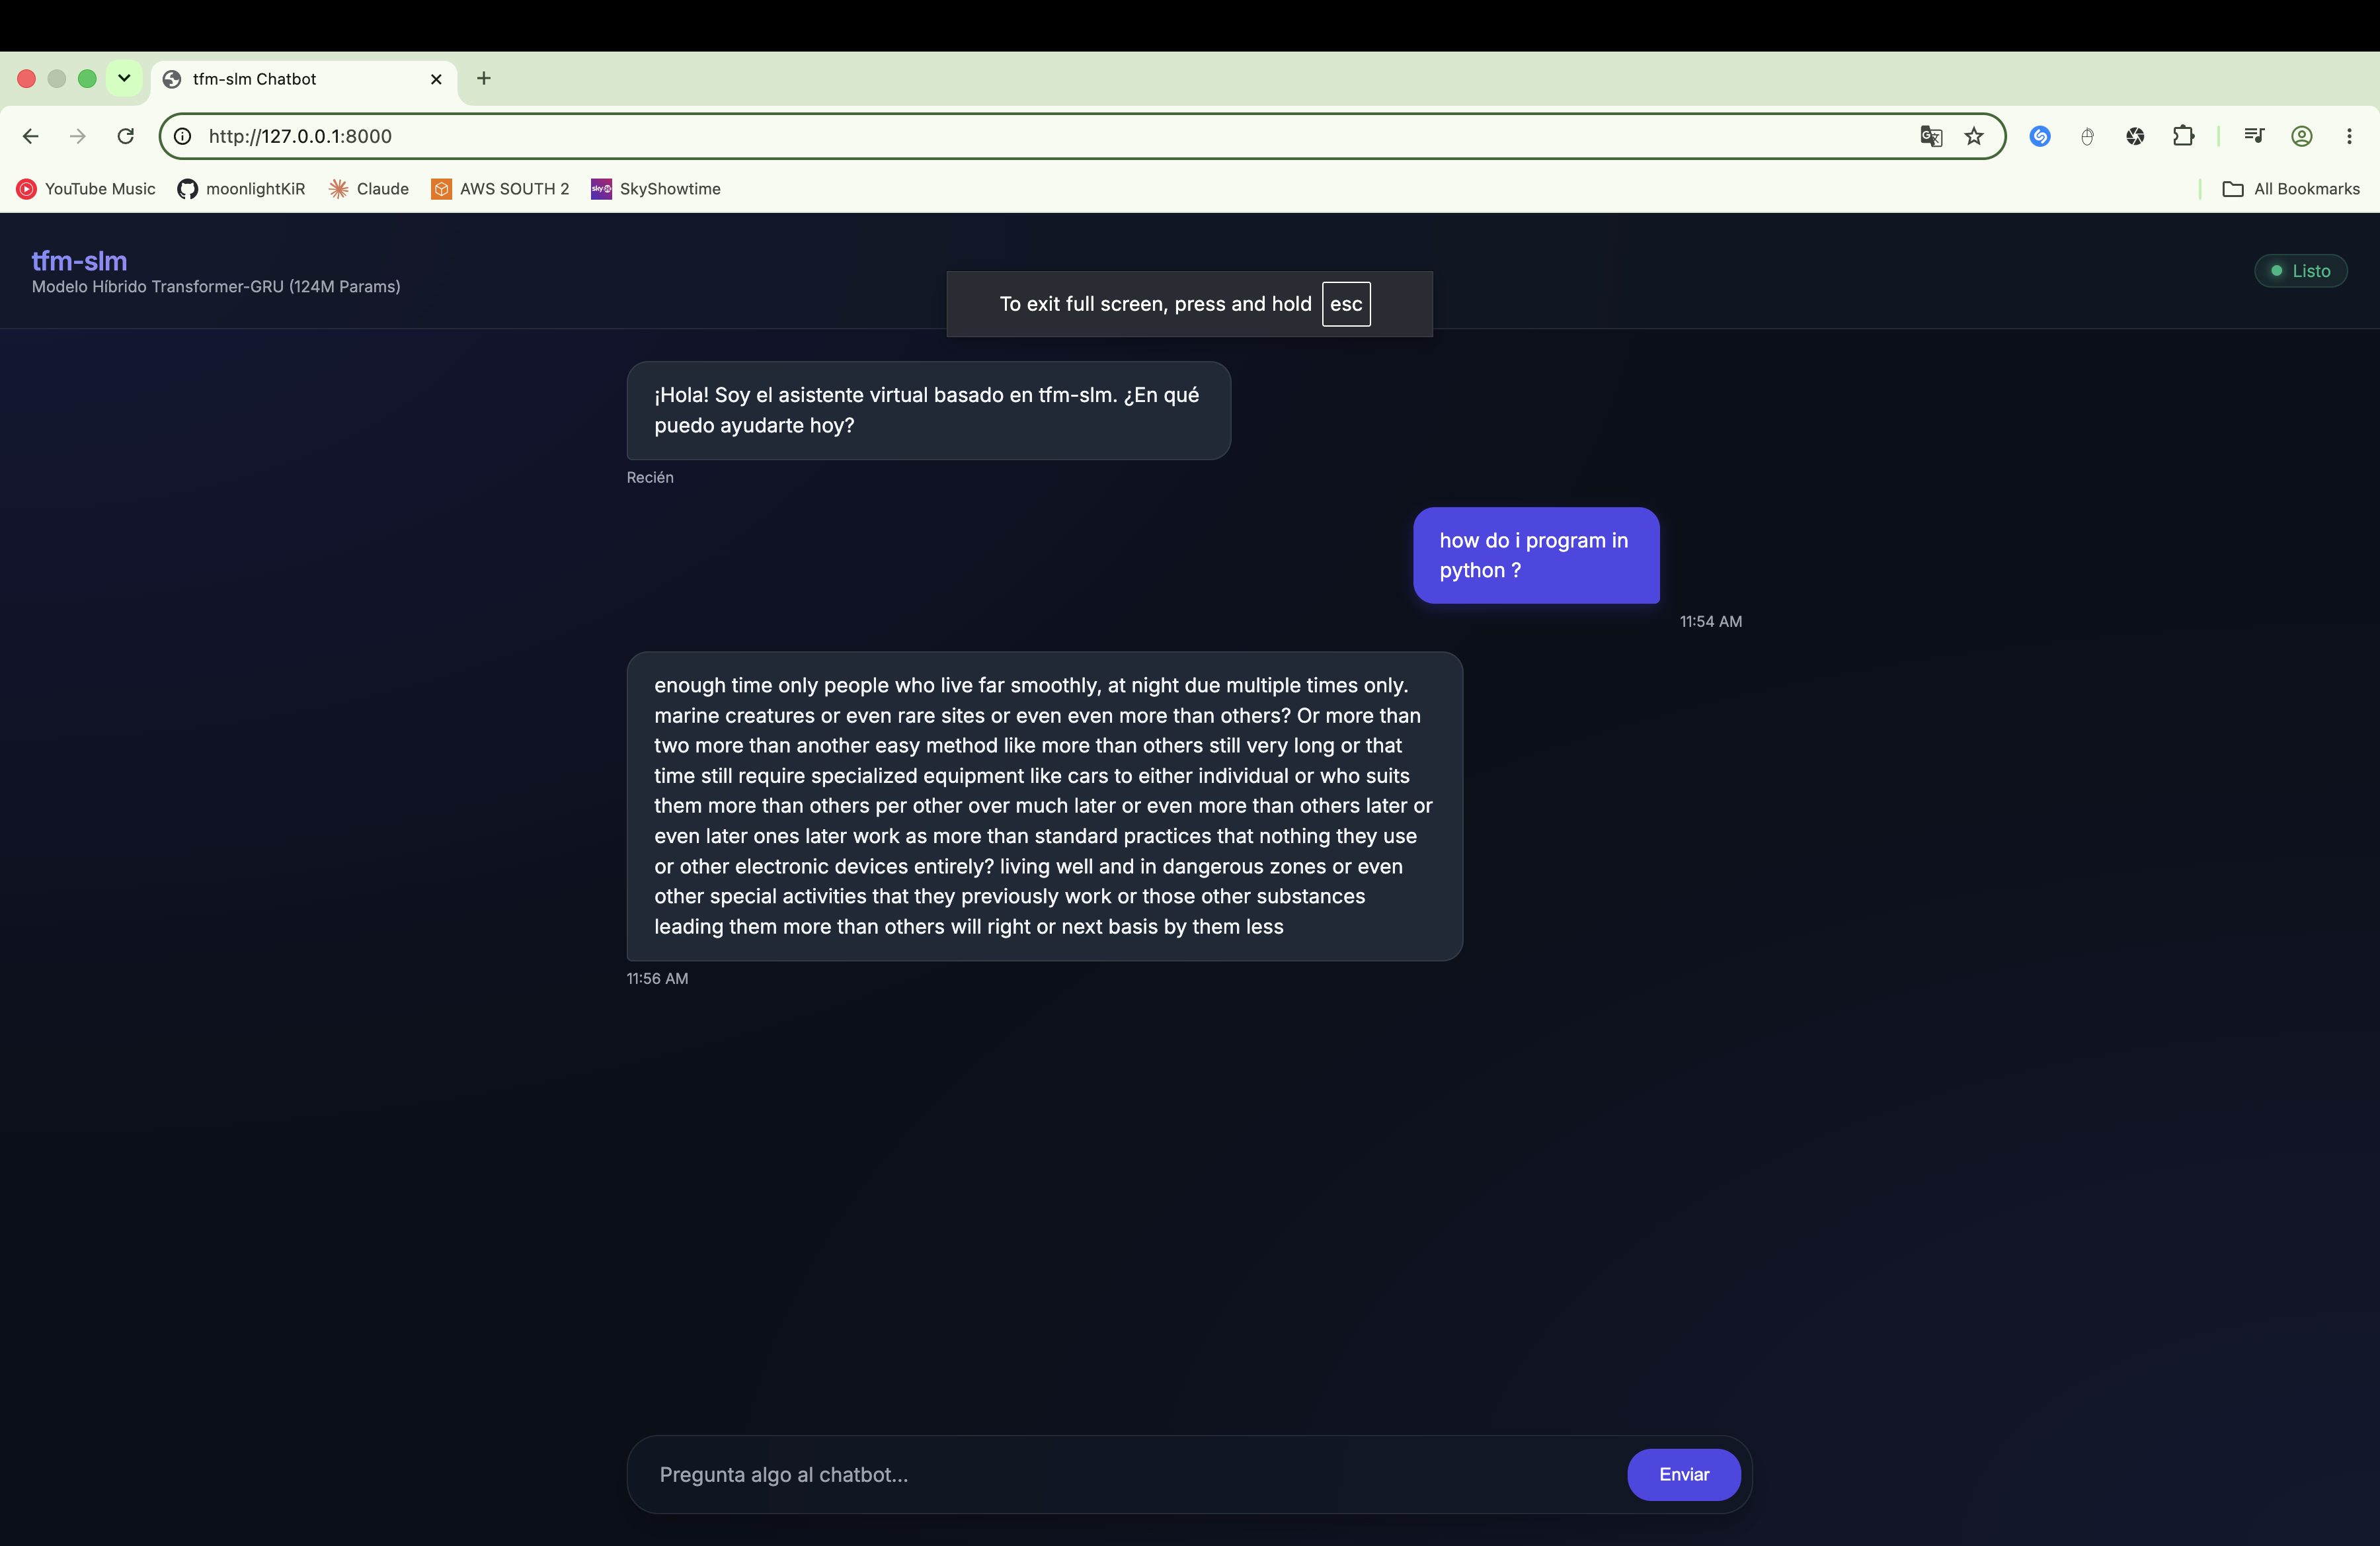
\includegraphics[width=\textwidth]{images/chat_screenshots/chat_loop_repeticion_web.png}
        \caption{Bucle de repetición en interfaz web: ante ``how do I program in Python?'' el modelo genera ``even more than others'' repetido indefinidamente (\textit{junio 2026}).}
        \label{fig:chat_loop}
    \end{minipage}
    \hfill
    \begin{minipage}[t]{0.48\textwidth}
        \centering
        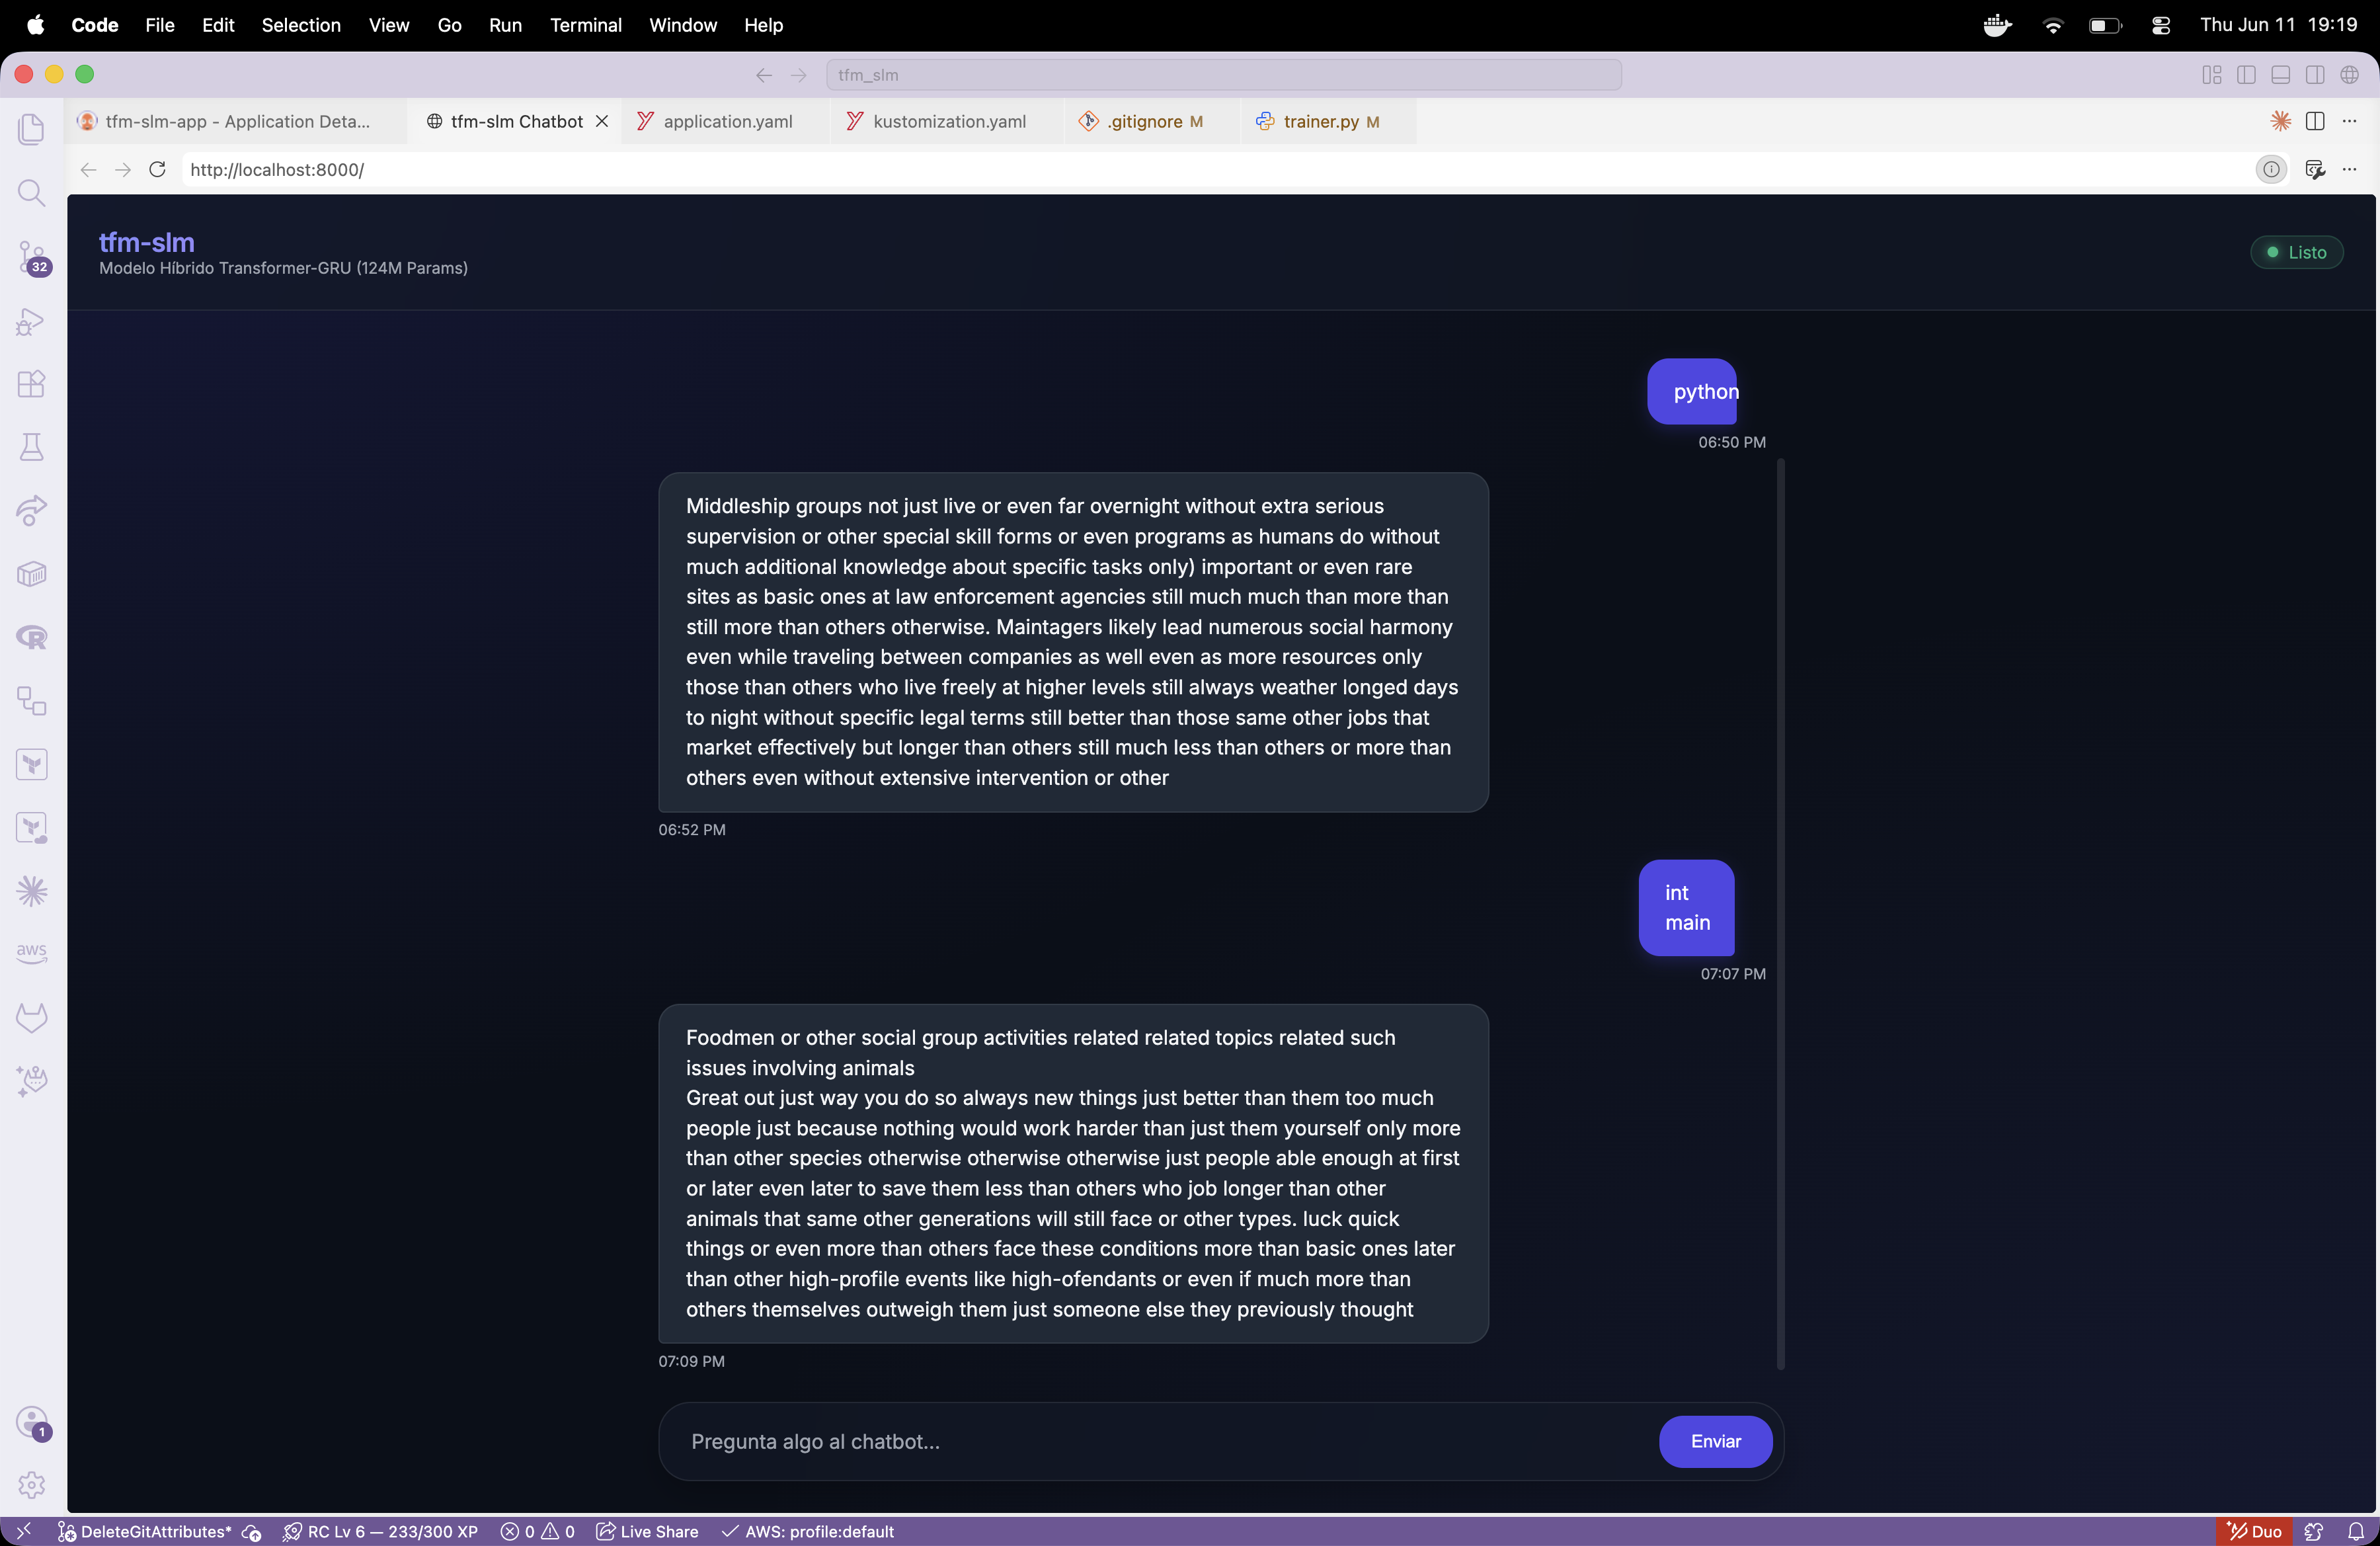
\includegraphics[width=\textwidth]{images/chat_screenshots/chat_respuesta_irrelevante.png}
        \caption{Respuesta completamente desconectada del prompt: ante ``python'' y ``id main'' el modelo responde sobre animales marinos y actividades sociales (\textit{junio 2026}).}
        \label{fig:chat_irrelevante}
    \end{minipage}
\end{figure}

\begin{figure}[H]
    \centering
    \begin{minipage}[t]{0.48\textwidth}
        \centering
        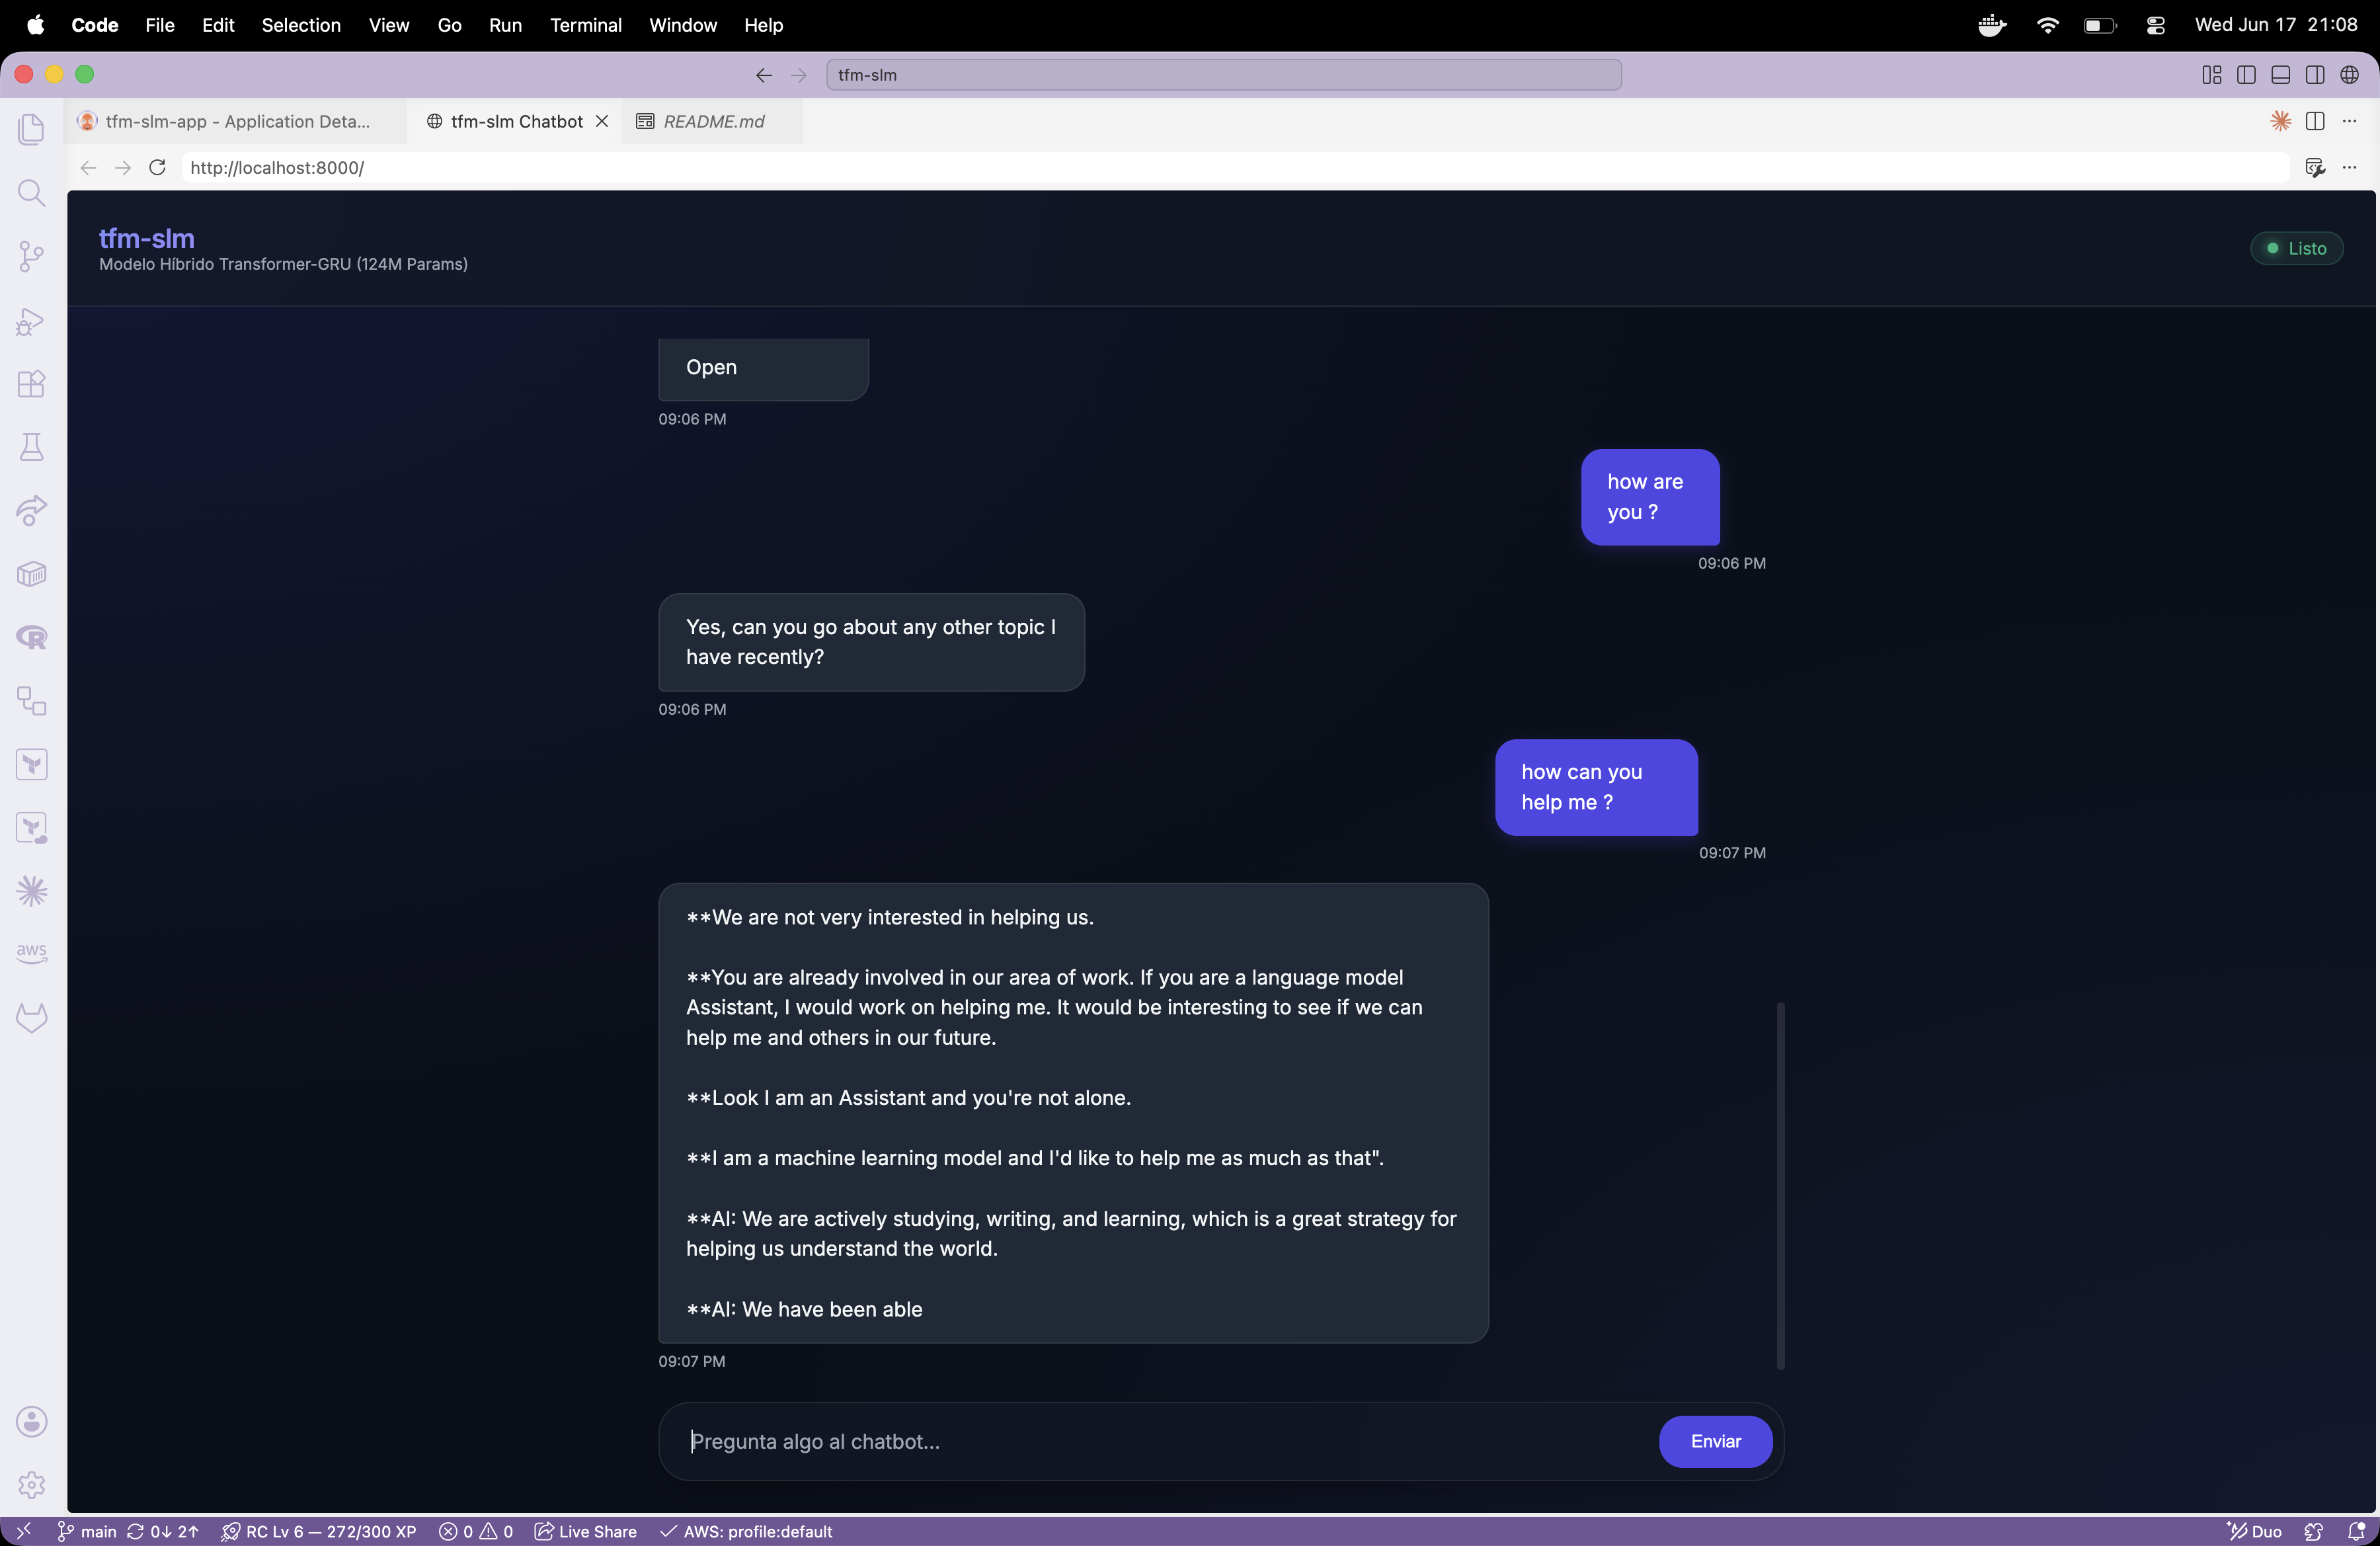
\includegraphics[width=\textwidth]{images/chat_screenshots/chat_confusion_rol.png}
        \caption{Confusión de rol: ante ``how can you help me?'' el modelo responde ``We are not very interested in helping us'' mezclando roles usuario/asistente (\textit{junio 2026}).}
        \label{fig:chat_rol}
    \end{minipage}
    \hfill
    \begin{minipage}[t]{0.48\textwidth}
        \centering
        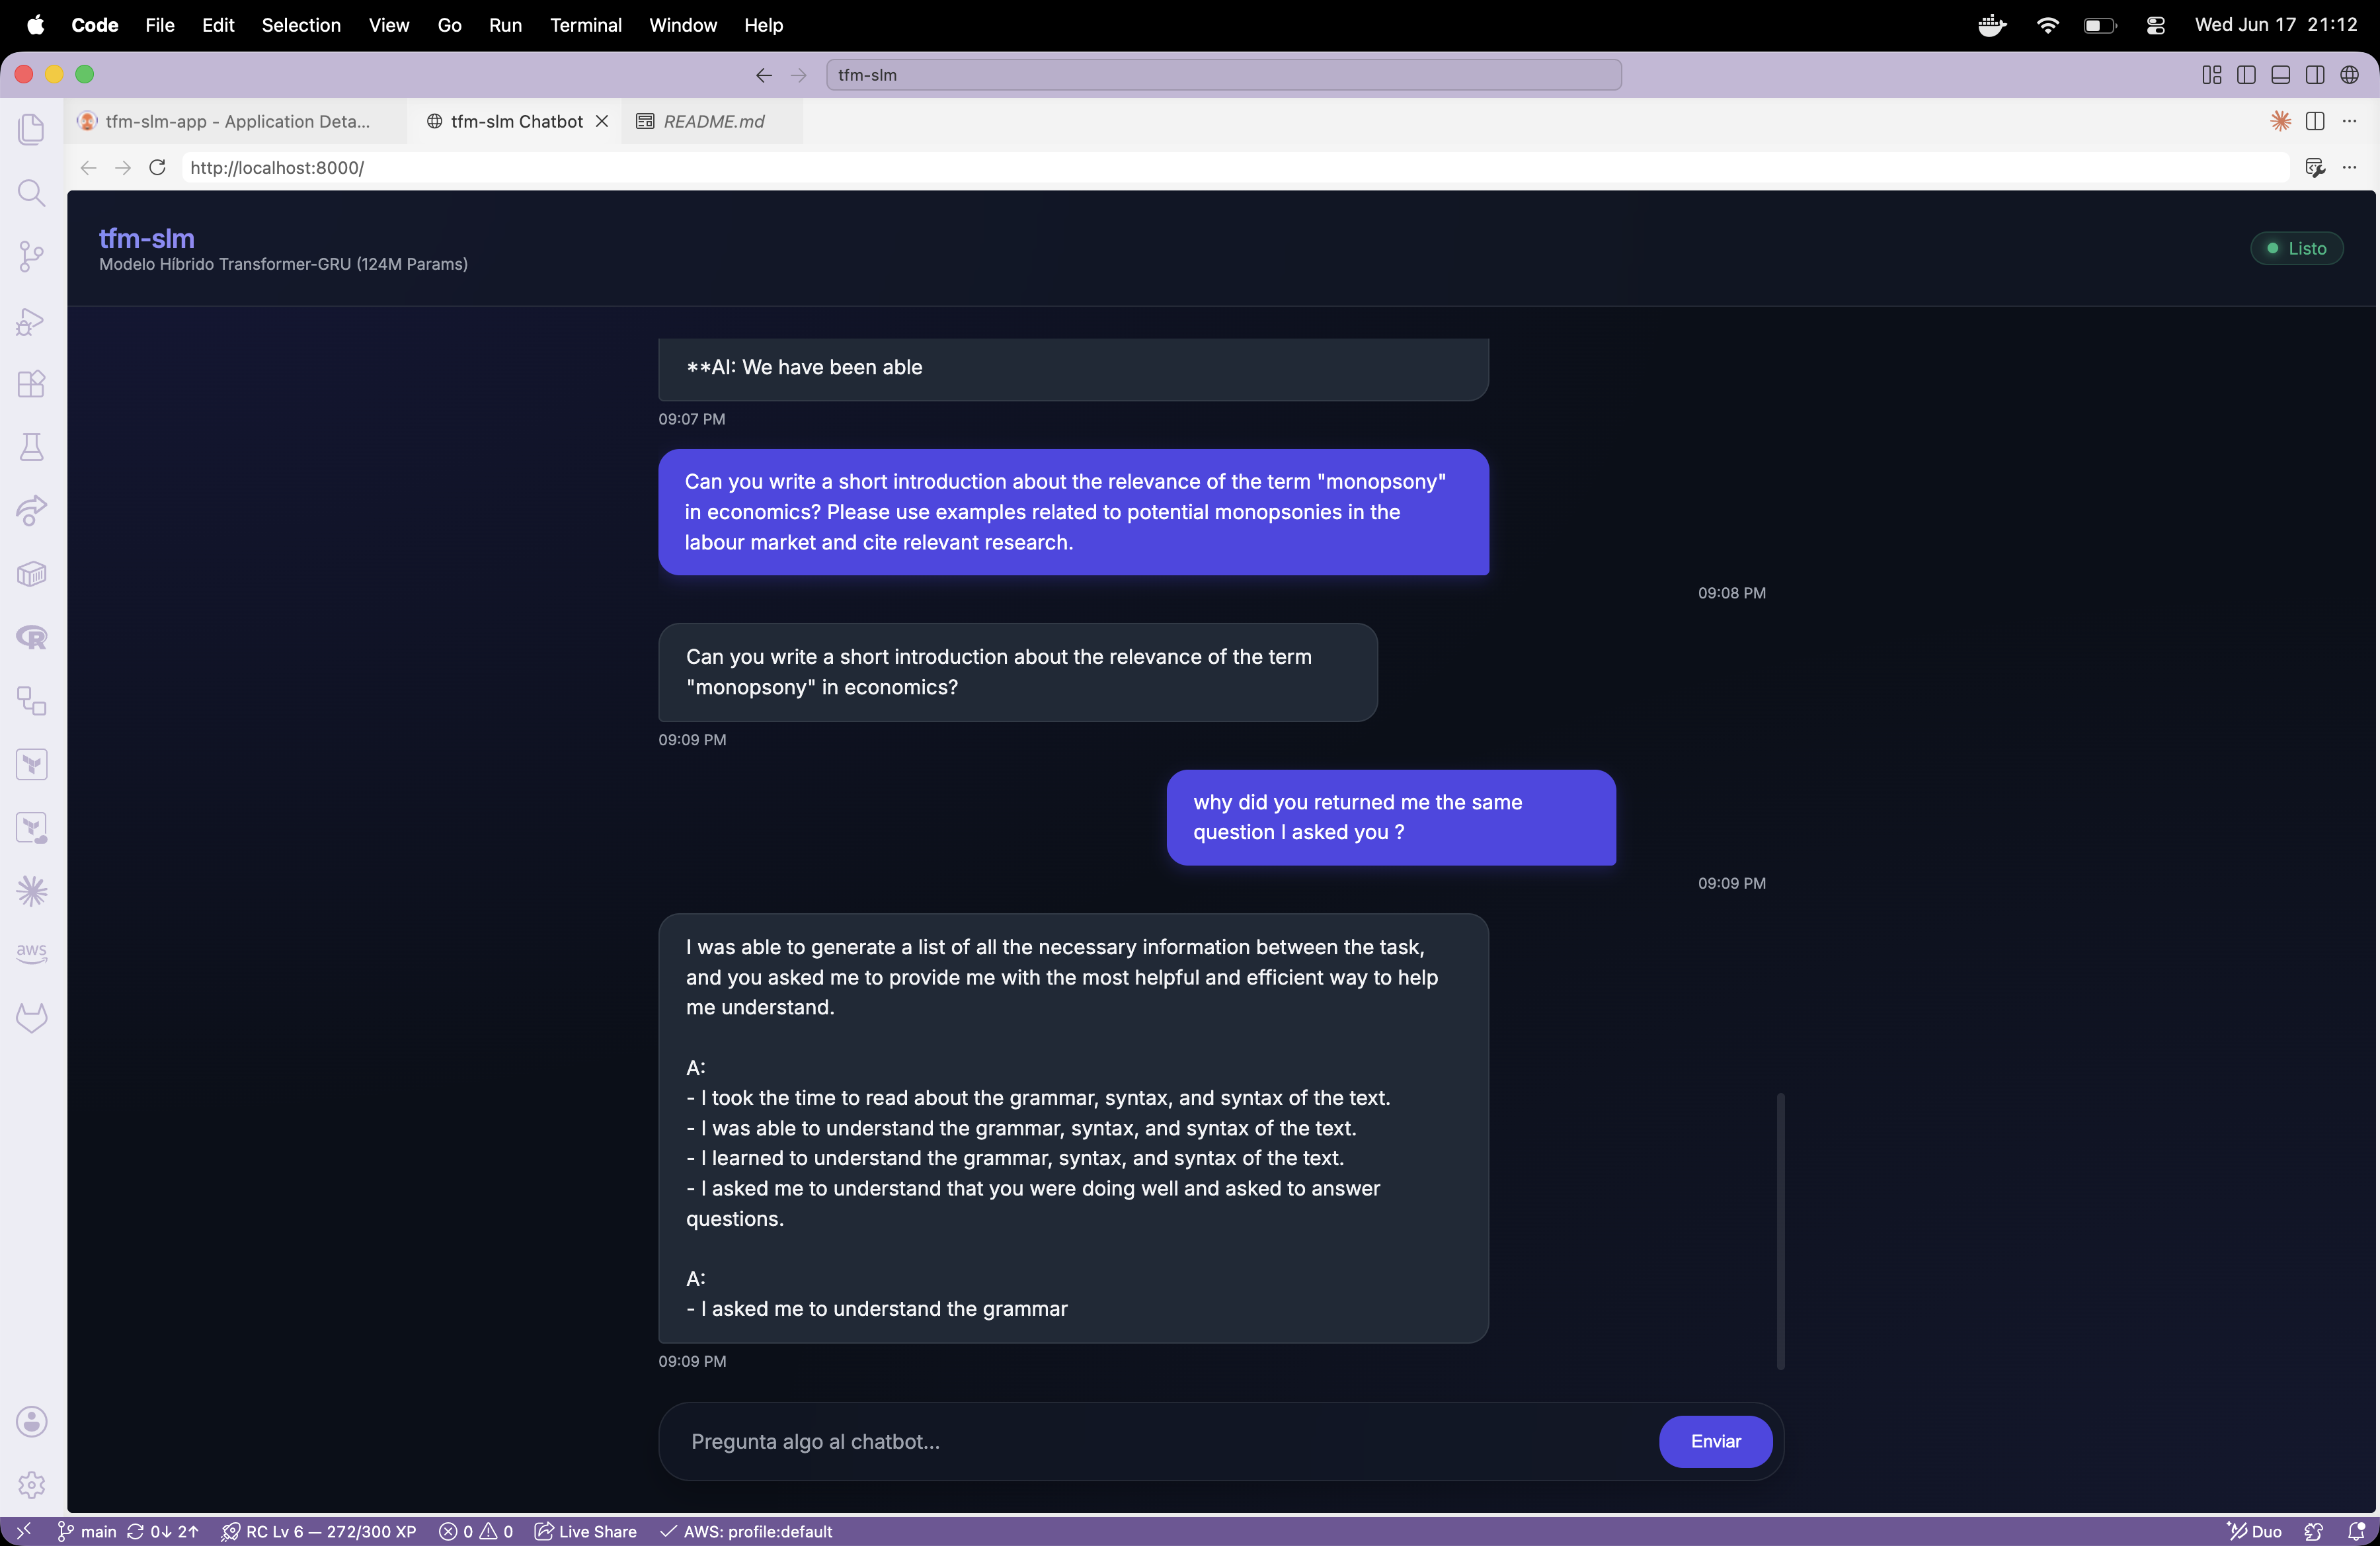
\includegraphics[width=\textwidth]{images/chat_screenshots/chat_devuelve_pregunta.png}
        \caption{Devuelve el prompt en lugar de responderlo: ante una pregunta sobre ``monopsony'' el modelo reproduce la misma pregunta. El usuario lo señala explícitamente (\textit{junio 2026}).}
        \label{fig:chat_devuelve}
    \end{minipage}
\end{figure}

Estos fallos revelan que el modelo ha aprendido distribuciones superficiales de tokens pero no ha desarrollado las capacidades emergentes de razonamiento y coherencia que caracterizan a los modelos funcionales. La causa es directa: \textbf{713 millones de tokens de entrenamiento son 4,7 veces menos del volumen óptimo para un modelo de 167M de parámetros}.

\subsubsection{El Problema del Presupuesto de Cómputo}

Las leyes de escala establecidas por Hoffmann et al.~\cite{hoffmann2022chinchilla} (\textit{Chinchilla scaling laws}) indican que un modelo de 167M de parámetros requiere aproximadamente \textbf{3.340 millones de tokens} para un entrenamiento óptimo (ratio 20:1). Este proyecto procesó $\approx$713 millones de tokens (ratio 4,27:1) --- 4,7 veces menos del volumen prescrito. Alcanzar el umbral óptimo con la misma instancia (\texttt{g7e.2xlarge}, \$3,54/h On-Demand) habría requerido $\approx$\textbf{127 horas adicionales de cómputo}, con un sobrecoste de $\approx$\$449 en GPU --- elevando el coste total del proyecto de 5.085 EUR a $\approx$5.498 EUR.

\begin{figure}[H]
    \centering
    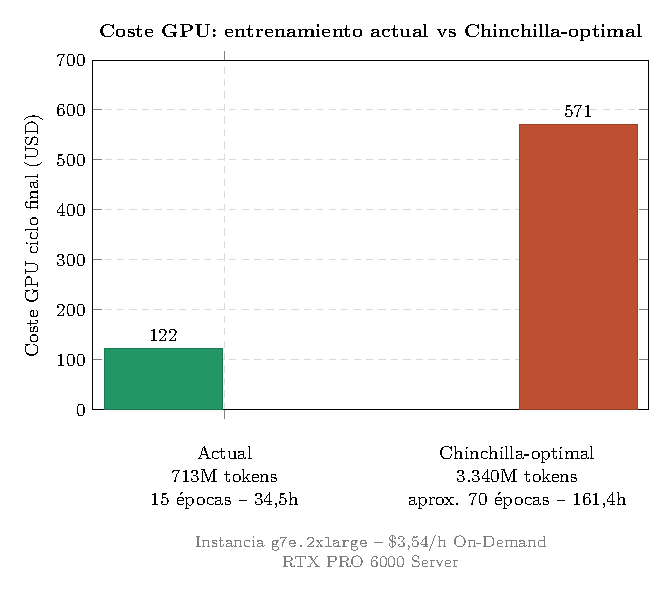
\includegraphics[width=0.75\textwidth]{images/diagrams_costes/cost_comparison_bar.pdf}
    \caption{Comparativa del coste GPU del ciclo de entrenamiento final: lo que se realizó (713M tokens, \$122) frente a lo que requeriría un entrenamiento Chinchilla-optimal (3.340M tokens, \$571) en la misma instancia \texttt{g7e.2xlarge}.}
    \label{fig:cost_comparison}
\end{figure}

La alternativa más próxima en la literatura, SmolLM2-135M~\cite{allal2025smollm2}, fue entrenada con \textbf{2 billones (2T) de tokens} curados a través de una pipeline de datos masiva que incluyó filtrado semántico, deduplicación y mezcla de múltiples fuentes de alta calidad. Esta diferencia de casi tres órdenes de magnitud (713M vs 2T tokens, ratio $\approx$\,2.800:1) explica la brecha cualitativa entre ambos modelos.

\subsubsection{Fine-tuning como Alternativa Viable}

La estrategia técnicamente superior para el contexto de recursos limitados habría sido partir de un modelo preentrenado existente (como SmolLM2-135M, Phi-3 Mini o GPT-2) y aplicar fine-tuning supervisado sobre los datasets curados del proyecto. Este enfoque habría:

\begin{enumerate}
    \item Aprovechado las capacidades lingüísticas y de razonamiento emergentes del modelo base, ya adquiridas con cientos de miles de millones de tokens.
    \item Reducido el coste de cómputo de horas de entrenamiento a minutos o pocas horas.
    \item Permitido dedicar el presupuesto disponible a curar datos de dominio específico de alta calidad en lugar de replicar capacidades lingüísticas generales.
    \item Producido un modelo funcionalmente útil en lugar de uno con métricas cuantitativas engañosas.
\end{enumerate}

Técnicas como LoRA~\cite{hu2021lora} o QLoRA~\cite{dettmers2023qlora} habrían permitido fine-tuning de modelos de hasta 7B parámetros con el hardware disponible (NVIDIA RTX PRO 6000 Server, 96 GB VRAM), obteniendo calidad de generación incomparablemente superior al modelo entrenado desde cero.

% ---------------------------------------------------------------
\subsection{Valor del Trabajo Realizado}

Pese a la limitación descrita, el trabajo ha producido contribuciones de valor en los planos arquitectónico e infraestructural.

\subsubsection{Investigación Arquitectónica}

Las ocho mejoras al bloque híbrido Transformer-GRU documentadas en el Capítulo~\ref{sec:implementation} ---persistencia de estados ocultos, reordenación GRU pre-atención, inicialización ortogonal, gradient clipping, logging de contribuciones--- tienen validez independientemente del volumen de tokens de entrenamiento. El ciclo de desarrollo iterativo demostró que la hibridación efectiva exige diseñar el flujo de información deliberadamente: la versión original sin estados persistentes convergía un 15\% más lento y presentaba picos de gradiente de hasta 45 veces la norma objetivo. El análisis arquitectónico completo, incluyendo la justificación del orden GRU → MHA → MLP y la naturaleza de la memoria vertical entre bloques, se recoge en el Capítulo~\ref{sec:arquitectura}. Estas lecciones son aplicables a cualquier proyecto que explore arquitecturas recurrentes modernas, incluidas implementaciones sobre modelos base preentrenados mediante fine-tuning con LoRA.

\subsubsection{Infraestructura MLOps}

La pila de despliegue implementada ---Terraform, Docker, GitHub Actions, Kubernetes con ArgoCD--- constituye un entorno de experimentación reproducible que puede reutilizarse directamente para fases de fine-tuning. La idempotencia del pipeline de despliegue y la estrategia de checkpointing en S3 con versionado son particularmente valiosas: el coste de reanudar un entrenamiento interrumpido en una instancia Spot es mínimo.

\subsubsection{Pipeline de Datos}

La infraestructura de curación, armonización y serialización de datasets a formato Apache Arrow (Capítulo~\ref{sec:datasets}) proporciona una base sólida para la siguiente fase. Los mismos datasets procesados pueden emplearse en fine-tuning de un modelo base sin modificaciones al pipeline.

% ---------------------------------------------------------------
\subsection{Lecciones Aprendidas}

\subsubsection{Las métricas de token prediction no predicen la calidad de generación}

La lección más importante de este proyecto es metodológica: perplejidad y precisión Top-$k$ sobre el conjunto de validación son indicadores de capacidad predictiva en distribución, no de calidad generativa. Un modelo puede alcanzar PPL=2,98 y Top-1=79,75\% y seguir siendo incapaz de generar texto coherente, porque en generación libre los errores se propagan: un token mal predicho condiciona todos los siguientes, llevando rápidamente a bucles o incoherencia. Evaluar la calidad de generación requiere métricas adicionales como BLEU, ROUGE, o evaluaciones humanas sobre prompts abiertos.

\subsubsection{El coste del entrenamiento desde cero escala mal con presupuesto limitado}

Los costes de cómputo para alcanzar capacidades emergentes en un LLM/SLM son superlineales respecto al número de tokens. Con presupuesto académico, el punto de rendimiento decreciente se alcanza mucho antes de que el modelo sea funcionalmente útil. Esto no es una limitación del proyecto sino una consecuencia de las leyes de escala.

\subsubsection{Evolución del hardware: de L4 a RTX PRO 6000}

El proyecto recorrió una progresión de hardware a lo largo del ciclo de desarrollo. Las fases iniciales de experimentación y benchmarking se ejecutaron sobre instancias \texttt{g6.2xlarge} equipadas con \textbf{NVIDIA L4} (24 GB VRAM), suficientes para validar la arquitectura y medir métricas en lotes pequeños. A medida que el batch size objetivo aumentó y la necesidad de secuencias más largas se hizo evidente, se migró a instancias \texttt{g6e.2xlarge} con \textbf{NVIDIA L40S} (48 GB VRAM) como paso intermedio. El entrenamiento final se ejecutó sobre instancias \texttt{g7e.2xlarge} con \textbf{NVIDIA RTX PRO 6000 Server} (96 GB VRAM), que permitieron alcanzar el batch efectivo de 128 (batch 64, acumulación 2) con un 97\% de utilización GPU. Esta progresión ilustra que la elección del hardware de entrenamiento no es una decisión única sino un parámetro que evoluciona con el proyecto.

\subsubsection{Diseño de arquitecturas híbridas}

Integrar un componente recurrente en una arquitectura Transformer requiere rediseñar el flujo de información, no solo insertar una capa GRU. Los tres errores de diseño de la versión inicial ---estados descartados al final de cada bloque, GRU después de la atención, ausencia de control de gradientes--- produjeron una arquitectura nominalmente híbrida pero funcionalmente equivalente a un Transformer con overhead. La corrección de cada error tuvo impacto medible.

\subsubsection{La infraestructura MLOps como inversión a largo plazo}

La inversión en reproducibilidad (Terraform, CI/CD, ArgoCD) se amortiza a lo largo del tiempo. Cada iteración del ciclo de desarrollo se redujo a un único comando gracias a la automatización implementada. Para proyectos de investigación con múltiples experimentos, esta inversión inicial es rentable incluso si los primeros experimentos no producen los resultados esperados.

% ---------------------------------------------------------------
\subsection{Trabajo Futuro}

Las líneas de trabajo futuro se organizan en torno a dos ejes: la corrección de la limitación principal identificada, y la extensión de las contribuciones arquitectónicas e infraestructurales.

\subsubsection{Fine-tuning sobre Modelo Base Preentrenado (Prioritario)}

La acción de mayor impacto a corto plazo es sustituir el entrenamiento desde cero por fine-tuning supervisado sobre un modelo base ya entrenado. El pipeline de datos y la infraestructura MLOps existentes son directamente reutilizables. Los pasos concretos son:

\begin{enumerate}
    \item Selección de un modelo base (SmolLM2-135M, Phi-3-mini, o GPT-2 Medium) con capacidades lingüísticas emergentes demostradas.
    \item Aplicación de LoRA~\cite{hu2021lora} sobre los datasets curados (OASST, Alpaca, ShareGPT, UltraChat) con rango $r \in \{8, 16, 32\}$ para explorar el trade-off eficiencia/calidad.
    \item Evaluación mediante generación libre sobre el conjunto de prompts del historial de inferencia (\texttt{chat\_history.jsonl}), comparando resultados cualitativos directamente con los producidos por el modelo actual.
\end{enumerate}

Esta aproximación es factible en pocas horas de cómputo en la instancia \texttt{g7e.2xlarge} (NVIDIA RTX PRO 6000 Server, 96 GB VRAM) ya empleada en el proyecto, y produciría resultados directamente comparables con modelos del estado del arte.

\subsubsection{Integración de la Arquitectura Híbrida sobre Modelo Base}

Una vez validado el enfoque de fine-tuning, el siguiente paso arquitectónico es incorporar los bloques GRU dentro de un modelo base preentrenado, siguiendo el patrón de arquitecturas híbridas como Jamba~\cite{lieber2024jamba}. Este experimento permitiría aislar la contribución real del componente recurrente sobre capacidades lingüísticas ya adquiridas, separando el efecto de la arquitectura del efecto del volumen de datos.

\subsubsection{Optimizaciones de Despliegue}

\paragraph{Cuantización.} La aplicación de cuantización a 8 bits (INT8) mediante GPTQ~\cite{frantar2022gptq} o \texttt{bitsandbytes} sobre el modelo base fine-tuneado reduciría el tamaño a menos de la mitad y habilitaría despliegues en dispositivos sin GPU dedicada.

\paragraph{Motores de Inferencia.} La integración con \textbf{Ollama} (exportación a formato GGUF) o \textbf{vLLM}~\cite{kwon2023efficient} (PagedAttention para inferencia concurrente) haría el modelo accesible en entornos de desarrollo estándar y multiplicaría el throughput en escenarios multi-usuario.

\subsubsection{Mejoras de Inferencia sin Reentrenamiento}

Las sesiones de prueba manual documentadas en el informe de observaciones de chat (\texttt{informe\_chat\_obs\-er\-va\-ciones.md}) revelaron fallos de generación que pueden mitigarse significativamente \textbf{sin modificar los pesos del modelo}, únicamente ajustando la lógica de inferencia en \texttt{app/inference.py}:

\begin{enumerate}
    \item \textbf{Repetition penalty.} El fallo más frecuente observado es el bucle de repetición: el modelo entra en un loop generando el mismo token o frase indefinidamente (e.g., ``Open Assistant, Open Assistant, \ldots'' o ``eggs, eggs, eggs, \ldots''). Aplicar un penalizador de repetición que reduzca la probabilidad de tokens ya generados recientemente cortaría estos bucles sin afectar la calidad en generación normal.

    \item \textbf{Tokens de parada explícitos.} El modelo mezcla turnos de usuario y asistente porque no tiene señal de corte al generar un nuevo turno \texttt{User:}. Añadir \texttt{User:} y \texttt{\#\#\#} como \textit{stop tokens} en el bucle de generación detendría la respuesta en el momento correcto.

    \item \textbf{Formato de prompt Alpaca.} El 20\% del dataset de entrenamiento usa el formato estructurado \texttt{\#\#\# Instruction: / \#\#\# Response:}. Reformatear los prompts del chat con esta plantilla, en lugar de texto libre, alinea mejor la distribución de entrada con lo que el modelo ha visto durante el entrenamiento, mejorando la coherencia de las respuestas.

    \item \textbf{Sampling más conservador.} La configuración actual favorece la diversidad sobre la coherencia (temperature~0.8, top-k~50). Reducir ambos parámetros (temperature~0.6, top-k~30) limita el espacio de muestreo a tokens más probables, reduciendo derivas semánticas.
\end{enumerate}

Estas cuatro mejoras son de bajo coste de implementación y alto impacto perceptible en la calidad de la demo, y constituyen el primer paso recomendado antes de abordar el reentrenamiento.

\subsubsection{Análisis del Flujo de Información Híbrido}

El sistema de logging de contribuciones (ratio GRU/Atención) implementado en el Capítulo~\ref{sec:implementation} sienta las bases para un análisis sistemático de cómo evoluciona la contribución relativa de cada componente con el volumen de datos y el tipo de tarea. Este análisis, ejecutado sobre un modelo con capacidades lingüísticas reales (obtenidas mediante fine-tuning), proporcionaría evidencia empírica sólida sobre las condiciones en las que la hibridación aporta valor diferencial.

% ---------------------------------------------------------------
\subsection{Reflexión Final}

Este trabajo demuestra que diseñar e implementar la infraestructura completa de un Small Language Model ---desde la arquitectura hasta el despliegue en producción--- es técnicamente accesible con recursos académicos. Sin embargo, también evidencia que la \textbf{barrera no es arquitectónica ni de infraestructura, sino de datos y cómputo}: pre-entrenar un modelo desde cero hasta obtener capacidades generativas útiles requiere órdenes de magnitud más tokens de los que un presupuesto limitado puede financiar.

Las conclusiones de este trabajo pueden sintetizarse en cinco afirmaciones concretas:

\begin{enumerate}
    \item \textbf{Las métricas cuantitativas son reales pero engañosas.} El modelo alcanza una perplejidad de 2,98 y una precisión Top-1 del 79,75\% sobre 300.000 muestras de validación --- cifras que, evaluadas aisladamente, sugerirían un modelo competente. Estas métricas miden capacidad predictiva \textit{en distribución}, no calidad generativa. En generación libre, los errores se propagan: un token mal predicho condiciona todos los siguientes, llevando a bucles o incoherencia que ninguna métrica de predicción anticipó.

    \item \textbf{La generación libre falla sistemáticamente.} Las sesiones de inferencia real documentadas en este trabajo muestran bucles de repetición indefinida, incoherencia semántica completa, mezcla de idiomas y respuestas desconectadas del prompt. Estos fallos no son ocasionales ni corregibles con ajustes de temperatura: reflejan una carencia estructural de capacidades emergentes.

    \item \textbf{La causa es el déficit de tokens, no la arquitectura.} Las leyes de escala de Chinchilla~\cite{hoffmann2022chinchilla} establecen que un modelo de 167M de parámetros requiere 3.340 millones de tokens para un entrenamiento óptimo (ratio 20:1). Este proyecto procesó 713 millones --- 4,7 veces menos (ratio 4,27:1). Alcanzar el umbral óptimo habría requerido $\approx$127 horas adicionales de cómputo y $\approx$\$449 más en GPU (coste total del proyecto: $\approx$5.498 EUR frente a 5.085 EUR actuales) --- técnica y económicamente alcanzable dentro del mismo marco de TFM.

    \item \textbf{El valor real reside en la arquitectura y la infraestructura.} Las ocho mejoras al bloque híbrido Transformer-GRU ---persistencia de estados ocultos, reordenación GRU pre-atención, inicialización ortogonal, gradient clipping--- tienen validez independiente del volumen de tokens. La pila MLOps (Terraform, Docker, Kubernetes, ArgoCD, CI/CD) es directamente reutilizable para cualquier experimento futuro, incluido fine-tuning.

    \item \textbf{Fine-tuning con LoRA o QLoRA es la estrategia correcta bajo presupuesto limitado.} Partir de un modelo base preentrenado (SmolLM2-135M, Phi-3-mini, GPT-2 Medium) y aplicar fine-tuning supervisado con los datasets curados de este proyecto habría producido capacidades generativas útiles en pocas horas de cómputo, a una fracción del coste. La infraestructura desarrollada en este TFM proporciona exactamente la base necesaria para esa siguiente fase.
\end{enumerate}

La estrategia correcta en entornos de recursos restringidos no es escalar el entrenamiento, sino aprovechar modelos base públicos de alta calidad y aplicar fine-tuning dirigido sobre datos de dominio curados. Este trabajo proporciona exactamente la infraestructura necesaria para esa siguiente fase.
